\documentclass[notes,color]{sepslide0}
\usepackage[overheads]{mysepslides}
\usepackage{graphicx,url,tikz}
\usepackage{scalalistings} % load last

\def\scalacolour{\color{violet}}

\title{Concurrent Programming: Introduction} 
\author{Gavin Lowe \\ with thanks to Bernard Sufrin}

\begin{document}

\begin{slide}
  
  \Title

\end{slide}
%%%%%%%%%%%%%%

\begin{slide}
\heading{Reading}

\begin{itemize}
\item Course notes.

\item Course textbook: Foundations of Multithreaded, Parallel, and Distributed
Programming, Gregory R. Andrews, Addison-Wesley, 2000.

\item
Alternative: Principle of Concurrent and Distributed Programming, M. Ben-Ari,
Prentice Hall, 1990.

\item Reading on Scala: \emph{Scala Tutorial},
  \url{https://www.scala-lang.org/docu/files/ScalaTutorial.pdf}; 
  \emph{Programming in Scala}, Odersky, Spoon and Venners; API documentation.
\end{itemize}
\end{slide}

%%%%%

\begin{slide}
\heading{Admin}

Three lectures per week in Weeks 1 and 2; two lectures per week in Weeks 3--7.

%% I will email you each week to recommend which chapters you study.  These will
%% be slightly front-loaded in term, but should finish in Week~7.  

Four problem sheets, discussed in four classes in Weeks 2, 4, 6, 8.

Six practical sessions, with four practical assignments: Weeks 2,
3, 4, 6, 7, 8.  You might need to work on practicals outside of practical
sessions.
\end{slide}

%%%%%

\begin{slide}
\heading{Prerequisites}

\begin{itemize}
\item Good programming skills using Scala. 

%% \item Basic understanding of object-oriented programming (objects, classes,
%% interfaces, inheritance, abstract classes, polymorphism), and comfort with
%% programming in Scala.

\item Familiarity with standard techniques for reasoning about (sequential)
programs:  pre- and post-conditions, invariants, and abstraction functions.
\end{itemize}

This course combines well with Concurrency (next term): Concurrent Programming
helps provide motivation for Concurrency, while Concurrency helps to provide
formal underpinnings for this course.
\end{slide}

%%%%%

\begin{slide}
\heading{Overview}

A concurrent program is any program consisting of multiple interacting tasks,
implemented as separate ``threads of control''.  The tasks may execute on the
same processor, on several close-coupled processors, or may be distributed
across a network.

The key concern is the correct sequencing of the interactions or
communications between tasks. 

%% Key concerns include:
%% %
%% \begin{itemize}
%% \item 
%% Correct sequencing of the interactions or communications between tasks;

%% \item 
%% Coordination of access to resources shared between tasks.  
%% \end{itemize}
\end{slide}

%%%%%

\begin{slide}
\heading{Processes and threads}

Concurrent tasks are  implemented as \emph{processes} and/or \emph{threads}.
%
\begin{itemize}
\item 
A thread is a single sequentially executing program.  
%% A thread is a ``single locus of control'' + a stack + an address space (all
%% that's needed to run a single sequential program). 
Several threads can share a single address space.  Threads sharing the same
address space can communicate with each
other using shared-memory.
%%  in a \textit{disciplined} way
They have a low communication overhead; context switching between threads can
be cheap.

\item
A process consists of one or more threads sharing an address space.  Distinct
processes have separate address spaces, protected from each other.  Processes
communicate with each other  using operating-system calls.  They have
relatively high communication overheads; context switching between processes
is expensive.
\end{itemize}
%

In this course we will use threads sharing a single address space.  However,
some of our programs use message passing (only), so the threads could be
replaced by processes in distinct address spaces.
%We will not differentiate much between threads and processes in this course.
\end{slide}

%%%%%

\begin{slide}
\heading{Reasons for concurrency: (1) speed}

Running a program on multiple processors concurrently will often make the
program faster.

Examples:
%
\begin{itemize}
\item
Scientific computations: e.g.~climate modelling, evolution of a galaxy,
effects of new drugs;

\item
Graphics and image processing;

\item
Combinatorial or optimisation problems: e.g.~scheduling problems, game-playing
algorithms.
\end{itemize}

Typical structures for such programs:
%
\begin{itemize}
\item
Data parallel: each thread/process works on part of the data, with all
threads/processes working in the same way;

\item
Task parallel: different threads/processes do different things.
\end{itemize}
%
% (Much more on this later.)
\end{slide}

%%%%%

\begin{slide}
\heading{Reasons for concurrency: (1) speed}

As we will see, using concurrency might not make a program faster.  There is a
danger that the communication and coordination costs outweigh the benefits of
using extra threads.
\end{slide}

%%%%%

\begin{slide}
\heading{Reasons for concurrency: (2) multi-task systems}

Many systems are responsible for a collection of independent (or
semi-independent) tasks, each with its own data.  Such systems are easier to
program using one single thread or process per task, rather than having a
single monolithic thread that is responsible for all the tasks.
\end{slide}

%%%%%

\begin{slide}
\heading{Reasons for concurrency: (2) multi-task  systems}

For example, consider a controller for a light, that turns the light on and
off periodically.  Using appropriate library code:
%
\begin{scala}
def controller(light: Light, tOn: Int, tOff: Int) = {
  private var tBase = getCurrentTime
  while(true){
    light.on; sleepUntil(tBase+tOn)
    light.off; sleepUntil(tBase+tOn+tOff); tBase = tBase + tOn + tOff
  }
}
\end{scala}

Now suppose you need to control 1000 lights.  
%
\begin{itemize}
\item
How would you do this with a sequential program?

\item
With a concurrent program it is easy: create one thread or process for each
light, and run them concurrently.
\end{itemize}
\end{slide}

%%%%%

\begin{slide}
\heading{Reasons for concurrency: (2) multi-task systems}

More examples:
%
\begin{itemize}
\item
Operating systems;

\item
Real-time controllers for factories, power plants, spacecraft, etc;

\item
Programs with GUIs that must respond to user actions;

\item
Simulations;

\item
Multi-character games.
\end{itemize}

In such multi-threaded multi-task systems, multiple threads or processes run
concurrently on the same processor(s), often with more threads/processes than
processors.  The threads/processes take turns to use the processor(s), under
the control of the operating system.
\end{slide}

%%%%%

\begin{slide}
\heading{Reasons for concurrency: (3) distributed computing}

Many applications make use of services provided by computers that are
physically distributed; these are necessarily concurrent.

Examples:
%
\begin{itemize}
\item 
The Web;

\item
File servers in a network;

\item
Database systems.
\end{itemize}

These applications often use a client-server architecture.

The components might themselves be multi-threaded.

Somewhat similarly, fault-tolerant systems may use redundant components.
\end{slide}

%%%%%%%%%%%%%%%%%%%%%%%%%%%%%%%%%%%%%%%%%%%%%%%%%%%%%%%%%%%%

\begin{slide}
\heading{Concurrent architectures}

We will briefly discuss a few different concurrent architectures, to provide
background for the rest of the course.
\end{slide}

%%%%%

\begin{slide}
\heading{Uni-processor multi-threaded systems}

Until early this century, most personal computers had a single processor.
However, they could run multiple (user and operating system) threads.

In such systems, the operating system is responsible for sharing the processor
between threads.  The operating system selects a suitable thread and
executes it until either:
\begin{itemize}
\item
the thread suspends itself, e.g.~waiting for input or output to complete; or

\item
the thread has used up its time allocation, at which point it is interrupted.
\end{itemize}
%
A new thread can then be scheduled.  See an Operating Systems textbook for
more details.
\end{slide}

%%%%%

\begin{slide}
\heading{Thread states}

%\includegraphics[width=12cm]{Pics/threadstates.eps}

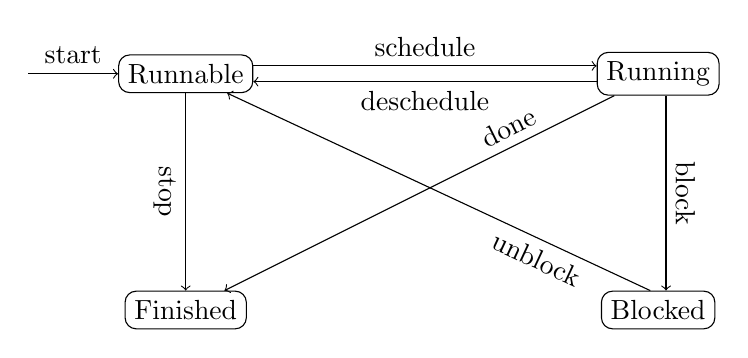
\begin{tikzpicture}
\draw(0,0) node[draw, rounded corners](runnable){Runnable};
\draw[<-] (runnable) -- node[above]{start} (-2,0);
%
\draw(6,0) node[draw, rounded corners](running){Running};
\draw[->] ([yshift = 1mm] runnable.east) -- node[above]{schedule} 
  ([yshift = 1mm] running.west);
\draw[->] ([yshift = -1mm] running.west) -- node[below]{deschedule} 
  ([yshift = -1mm] runnable.east);
%
% \draw (3,3) node[draw, rounded corners](waiting){Waiting};
% \draw[->] (running) -- node[above, sloped]{\scalashape wait} (waiting);
% \draw[->] ([xshift = -1mm] waiting.south) -- node[above, sloped]
%   {\scalashape notify} ([xshift = -1mm] runnable.north);
% \draw[->] ([xshift = 1mm] waiting.south) -- node[below, sloped]
%   {spurious wake-up} ([xshift = 1mm] runnable.north);
%
\draw (0, -3) node[draw, rounded corners](finished){Finished};
\draw[->] (runnable) -- node[below, sloped]{stop} (finished);
\draw[->] (running) -- node[above, sloped, near start]{done} (finished);
%
\draw(6, -3) node[draw, rounded corners](blocked){Blocked};
\draw[->] ([xshift = 1mm] running.south) -- 
  node[above, sloped]{block} ([xshift = 1mm] blocked.north);
\draw[->] ([xshift = -1mm] blocked.north) -- 
  node[below, sloped, near start]{unblock} 
  ([xshift = -1mm] runnable);
%
% \draw(7, 3) node[draw, rounded corners](IOblocked){IO Blocked};
% \draw[->] ([xshift = -1mm] running.north) -- 
%   node[above, sloped]{block for IO} ([xshift = -1mm] IOblocked.south);
% \draw[->] ([xshift = 1mm] IOblocked.south) -- node[below, sloped]{complete IO} 
%   ([xshift = 1mm] running.north);
\end{tikzpicture}
\end{slide}

%%%%%

\begin{slide}
\heading{Shared-memory multiprocessors}

In shared-memory multiprocessors, several processors share one or more
memories.  They are connected by an interconnection network, e.g.\ a memory
bus.  Each processor has its own (fast) cache memory. 
%
\begin{center}
\ \includegraphics[width=6cm]{Pics/multiprocessors.eps}\ 
\end{center}
% \framebox{Fig 1.2 from Andrews}
% 
The shared memory might be organised hierarchically, particularly in a system
with many processors.
\end{slide}

%%%%%

\begin{slide}
\heading{Cache consistency}

In shared-memory multiprocessor systems, each processor has its own cache.
Values read from the main memory are copied into the cache; a subsequent read
of the same address will read that value from the cache.  If an address is
written to, that write initially happens just in the cache, and later copied
back to the main memory.

Different processors may read and write the same location.  This can be
problematic if the different caches are not consistent.  The specification of
most programming languages include a \emph{memory model} which defines the
degree of consistency that is guaranteed: see later.

%% It is therefore important to keep different caches consistent.  See the
%% Architecture course for details.
\end{slide}

%%%%%

{\advance\slideheight by 3mm
\begin{slide}
\heading{Multi-core processors}

Nowadays, most processors have multiple cores on the same chip.  Each core may
have its own level~1 cache, and they may share a level~2  and level-3 cache.
%
\begin{center}
\includegraphics[height=32mm]{190px-Dual_Core_Generic.svg.ps} \hspace{2cm}
(Image from Wikipedia.)
\end{center}

Most current off-the-shelf computers are dual-core or quad-core; servers
typically have tens or hundreds of cores.

Multi-core processors provide little speed-up unless the software is designed
to exploit concurrency.
\end{slide}}

%%%%%

\begin{slide}
\heading{General-purpose computing on graphics processing units}

A \emph{graphics processing unit} (GPU) is a special-purpose multi-core
processor, originally designed to do graphics processing.  They were designed
to perform many operations in parallel, and so are much faster at floating
point calculations than traditional
CPUs.\footnote{\url{http://gpgpu-computing.blogspot.com/}} 

They originally had rather limited functionality.  However, APIs have
been developed that allow them to be used for general-purpose computing.  They
have been used to parallelise many different
applications.\footnote{\url{http://en.wikipedia.org/wiki/GPGPU}} 

\vfill
\end{slide}

%%%%%

%{\advance\slideheight by 3mm
\begin{slide}
\heading{Distributed-memory systems}

In distributed-memory systems, each processor has its own private memory.
Processors communicate by message passing, rather than using shared memory. 
%
\begin{center}
\ \includegraphics[width=6cm]{Pics/distributed.eps}\ 
\end{center}
% \framebox{Fig 1.3 from Andrews}
%
They might communicate via a high-speed interconnection network, or over a
network, such as a local area Ethernet or the Internet.
\end{slide}

%%%%%

%% \begin{slide}
%% \heading{Distributed-memory multicomputers and networks}

%% A \emph{multicomputer} is a distributed-memory system where the processors are
%% physically close, connected by a high-speed interconnection network.

%% In \emph{network systems} (sometimes known as grids), processors
%% communicate over a network, such as a local area Ethernet or the
%% Internet.

%% One can, of course, build distributed-memory systems, where each computer is
%% itself a shared-memory multiprocessor.
%% % multicomputers from shared-memory multiprocessors.
%% \end{slide}

%% %%%%%

%% \begin{slide}
%% \heading{Grid systems and cloud computing}

%% Grid systems are large network systems, often sharing resources across
%% organisations.  They come in two main flavours:
%% %
%% \begin{description}
%% \item[Computational grids,] where computers work together on some
%%   computational task.
%%   % mostly used on problems that require little communication between the
%%   % subtasks. 

%% \item[Data grids,] where there is a huge amount of data to be processed.
%%   % Example types of data include the web (e.g.~web searching), astronomical
%%   % data, data from particle accelerators, genomic sequences.  The data grid may
%%   % be combined with a computational grid that operates on the data.
%% \end{description}


%% Cloud computing can be thought of as ``grids for hire''.  Companies ---such as
%% Amazon, HP, Google, Rackspace--- make grids of computers available to be hired
%% by organisations.  Whether to own your own grid or to hire is mainly an
%% economic decision. 
%% \end{slide}

%%%%%

%% \begin{slide}
%% \heading{Example: Google}

%% Google has 15 data centres worldwide, using about 900,000 servers.
%% %  between 500,000 and several
%% % million processors in total, grouped into clusters of a few thousand
%% % processors.\footnote{{\it Data-Intensive Supercomputing: The case for DISC},
%% %   Randal E. Bryant, CMU-CS-07-128.}
%% Each data centre stores several copies of the web (about 1.2 million terabytes)
%% % (about 200 terabytes),
%% together with indexes to allow efficient searching.  This is continually
%% updated by processes that crawl the web.

%% They use their own custom file system\footnote{{\it The Google File System}, 
%% Sanjay Ghemawat, Howard Gobioff, and Shun-Tak Leung,
%% \url{http://labs.google.com/papers/gfs.html}.}, to distribute the data across
%% servers, providing high performance and fault tolerance. 

%% Each web search uses about 1000 computers, in order to complete the search in
%% about 0.2 seconds.  

%% % Each web search requires about 10 seconds of computer time, but is completed
%% % in about 0.1 seconds by using multiple processors.

%% Their design uses hardware that is low-cost and low-power, rather than fast or
%% reliable. 

%% \vfill
%% \end{slide}

%%%%%

\begin{slide}
\heading{Shared variables}

We will mainly consider programs for shared-memory multiprocessors in this
course.

The main difficulty we have to overcome is ensuring \emph{disciplined} access
to shared variables.  

The following example shows what can happen if you allow undisciplined access.
Such programs are very hard to reason about.
\end{slide}

%%%%%

{\advance\slideheight by 3mm
\begin{slide}
\heading{A shared variable program}

\begin{scala}
import ox.scl._

/** Program to show the dangers of undisciplined shared variables. */
object Race{
  var x = 0

  /** Thread to increment x 1000 times. */
  def p = thread{ for(i <- 0 until 1000) x = x+1 }

  /** Thread to decrement x 1000 times. */
  def q = thread{ for(i <- 0 until 1000) x = x-1 }

  /** Parallel composition. */
  def system = p || q

  def main(args : Array[String]) = { run(system); println(x) }
}
\end{scala}% File Race/Race.scala
\end{slide}}


% \begin{selfnote}
% Reminder about tutorial.

% Scala built on top of Java; can use Java libraries; compiled into bytecode for
% execution on the Java Virtual Machine.  Influenced by Haskell.

% An object is basically a class with a single instance, sometimes called a
% \emph{singleton object}.  Most main modules in Scala are objects.

% Most typing is optional.  Needed with arguments of procedures, and recursion.
% Recommended when it improves clarity.

% \SCALA{var} for variables.  \SCALA{val} for constant values.  \SCALA{def} for
% definitions, e.g.~of procedures.  

% \SCALA{0 until 1000} means $[0 .. 1000)$.  
% \end{selfnote}


%%%%%

\begin{slide}
\heading{Basics of SCL}

\begin{itemize}
\item
SCL (Scala Concurrency Library) is a library of concurrency primitives.  It is
heavily based on CSO (Communicating Scala Objects), produced by Bernard
Sufrin.

\item \SCALA{thread\{<code>\}} defines a thread that when executed will
  execute \SCALA{<code>}.

\item It is also possible to use \SCALA{thread(name)\{<code>\}} to give the
  thread a name |name|.

\item The type |ThreadGroup| represents the parallel composition of zero or
  more threads.

\item If \SCALA{p} and \SCALA{q} are |ThreadGroup|s, then \SCALA{p || q}
  represents their parallel composition.  The parallel composition terminates
  when both threads have terminated.

\item If \SCALA{p} is a |ThreadGroup|, then |run(p)| or |p.run|
  runs~\SCALA{p}.
\end{itemize}
\end{slide}

%%%%%

\begin{slide}
\heading{Shared variables}

When the program \SCALA{Race} is executed, it doesn't always give $0$.  In
fact, it can give any answer between $-1000$ and $+1000$.  Why?
\end{slide}

%%%%%

\begin{slide}
\heading{Abstract model of concurrent execution}

Certain actions can be considered \emph{atomic}, e.g.~single (virtual) machine
instruction.

A sequential program executes a sequence of atomic actions.

A concurrent program runs two or more sequential programs, whose atomic
actions may be interleaved.  

Two actions are \emph{independent} if their order may be reversed without
changing the overall effect: for example, two actions concerning distinct
variables, or two reads of the same variable.  Interleaving of independent
atomic actions is not problematic.

However, interleaving of non-independent atomic actions can be problematic:
for example two writes of the same variable, or a read and a write of the same
variable. 
\end{slide}

%%%%%

\begin{slide}
\heading{Example}

Suppose \SCALA{x = x+1} is implemented by \SCALA{LD x; INC; ST x}, and 
\SCALA{x = x-1} is implemented by \SCALA{LD x; DEC; ST x}.  

The interleavings give three distinct results, starting from |x = 0|:
%
\begin{center}
\begin{tabular}{lccccccl}
\SCALA{x = x+1} & \SCALA{LD x} & \SCALA{INC} & \SCALA{ST x} & \\
\SCALA{x = x-1} &      &      &     & \SCALA{LD x} & \SCALA{DEC} & \SCALA{ST x}
& (\SCALA{x = 0}) 
\\
\hline
\SCALA{x = x+1} & \SCALA{LD x} &      & \SCALA{INC} & \SCALA{ST x} & \\
\SCALA{x = x-1} &      & \SCALA{LD x} &     &      & \SCALA{DEC} & \SCALA{ST x}
& (\SCALA{x = -1}) 
\\
\hline
\SCALA{x = x+1} & \SCALA{LD x} &      &     &      & \SCALA{INC} & \SCALA{ST x} & \\
\SCALA{x = x-1} &      & \SCALA{LD x} & \SCALA{DEC} & \SCALA{ST x} &     &
& (\SCALA{x = 1})
\end{tabular}
\end{center}

The different threads run at different rates depending on processor load,
scheduler whim, etc.  Predicting which interleaving will occur is effectively
impossible. 
\end{slide}

%%%%%

\begin{slide}
\heading{Caching}

Multiprocessor machines may cache variables.  But Java does not guarantee that
the caches will always be kept coherent.  Two concurrent threads may operate
independently on their own cached copies of the same variable!

%% Variables may be marked as \emph{volatile}:
%% \begin{scala}
%% @volatile var x : Int = 0;
%% \end{scala}
%% in which case it is flushed from the cache after writing, and reloaded from
%% memory on reading.  But that makes performance much slower!
\end{slide}

%%%%%

\begin{slide}
\heading{Compiler optimisations}

Consider the code
%
\begin{scala}
answer = <some value>
done = true
\end{scala}
%
It might seem reasonable for some concurrent thread to assume that if
\SCALA{done} is |true| then the assignment to \SCALA{answer} has occurred; for
example:
%
\begin{scala}
while(!done){ } // Busy wait.  Don't do this!!!
myAnswer = answer
\end{scala}
%
However, the compiler is allowed to reorder instructions, according to certain
rules, for example reordering the first code to
%
\begin{scala}
done = true
answer = <some value>
\end{scala}
\end{slide}

%%%%%

\begin{slide}
\heading{Disciplined interaction}

Programs that share variables in an undisciplined way are likely to be very
hard to reason about, unpredictable --- and wrong!

We define a \emph{race condition} to be where two non-independent actions can
occur in either order, with at least one of the orders leading to an incorrect
outcome.

A major goal in concurrent programming is to avoid race conditions. 
\end{slide}

%%%%%

\begin{slide}
\heading{Disciplined memory access}

If two threads concurrently perform non-independent actions on memory
locations, that normally constitutes a race condition, known as a \emph{memory
  race}.  In this course, we avoid \emph{all} such memory races.  (Formally we
will require a synchronisation between any two non-independent memory
actions.)

Avoiding such memory races has the additional benefit of removing the
types of errors introduced by caching or compiler optimisations: see later.

In the first part of the course, threads will use disjoint variables, except
for reading.  This avoids all memory races.

(The fourth year course Concurrent Algorithms and Data Structures adopts a
different view, allowing such concurrent actions.)
\end{slide}

%% Programming Languages and Operating Systems provide mechanisms to support
%% concurrent operation and disciplined inter-task interaction.  These should be
%% easy to reason about, preferably in a formal way.

%% \begin{slide}
%% \heading{Disciplined interaction}

%% In the first part of this course, we will adopt the following
%% discipline:\footnote{We will weaken this slightly later.}
%% %
%% \begin{quote}
%% Processes will use disjoint variables, except if both only read the variable.
%% \end{quote}


%% But then how can processes interact with one another?

%% \vfill
%% \end{slide}

%%%%%

\begin{selfnote}
NSA have issued a report saying that race conditions are the eighth most
dangerous programming error.
\end{selfnote}

%%%%%

\begin{slide}
\heading{Correctness properties} 

\begin{description}
\item[Safety/correctness:] The results produced by the program are correct.
  Typically this requires that the system state will satisfy an (intended)
  invariant property after every ``action''.

\item[Liveness/progress:] The system as a whole does something useful.
\end{description}

\bigskip

\heading{Performance properties}

\begin{description}
\item[Latency:]
Requests get serviced reasonably quickly.

\item[Throughput:]
The system deals with a high number of requests.
\end{description}
\end{slide}

%%%%%

\begin{slide}
\heading{Summary}

\begin{itemize}
\item
Processes and threads;

\item
Reasons for concurrency;

\item
Concurrent architectures;

\item
Shared variable programs; 

\item
Basics of SCL;

\item
Independent and non-independent actions, race conditions, disciplined
interaction; 


\item
Desirable properties.
\end{itemize}
\end{slide}




\end{document}
